\documentclass[tikz,border=2pt]{standalone}
\usepackage{amsmath}
\usepackage{pgfplots}
\pgfplotsset{compat=1.18}
\usetikzlibrary{arrows.meta}
\begin{document}
% Gains X in {0,2} with probability 1/2 each and Y = 1 surely: int_0^t F_X = t/2 on [0,2], t-1 afterwards;
% int_0^t F_Y = (t-1)_+. The X curve is never below the Y curve, so Y second-order dominates X.
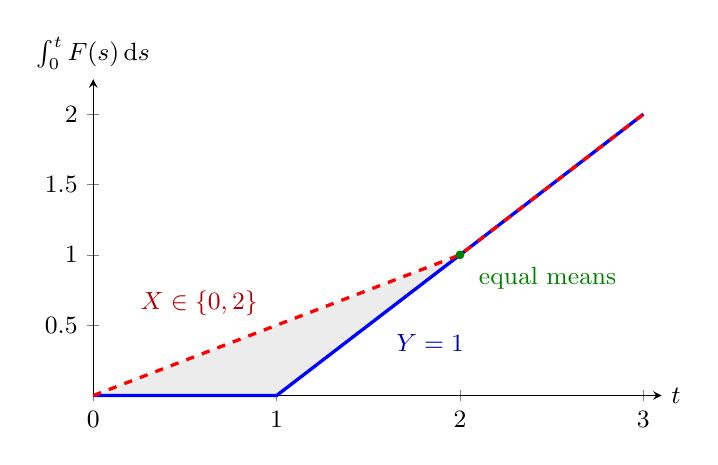
\begin{tikzpicture}[font=\small, >={Latex[length=2mm]}]
  \begin{axis}[
    axis lines=left, xmin=0, xmax=3.1, ymin=0, ymax=2.25,
    xtick={0,1,2,3}, ytick={0.5,1,1.5,2},
    xlabel={$t$}, ylabel={$\int_0^tF(s)\,\mathrm{d}s$},
    xlabel style={at={(axis description cs:1,0)}, anchor=west},
    ylabel style={rotate=-90, at={(axis description cs:0,1)}, anchor=south},
    width=8.8cm, height=5.6cm, clip=false
    ]
    \addplot[fill=gray!15, draw=none] coordinates {(0,0) (1,0) (2,1) (0,0)};
    \addplot[blue, very thick] coordinates {(0,0) (1,0) (3,2)};
    \addplot[red, very thick, dashed] coordinates {(0,0) (2,1) (3,2)};
    \node[red!70!black, anchor=south east] at (axis cs:0.95,0.5) {$X\in\{0,2\}$};
    \node[blue!70!black, anchor=north west] at (axis cs:1.6,0.5) {$Y=1$};
    \fill[green!50!black] (axis cs:2,1) circle (1.6pt);
    \node[green!50!black, anchor=north west] at (axis cs:2.05,0.98) {equal means};
  \end{axis}
\end{tikzpicture}
\end{document}
